% Specify what kind of document this is
\documentclass[10pt, letterpaper]{article}


% Load extra packages to get access to special symbols and commands
\usepackage{fullpage}
\usepackage{color}
\usepackage{amsmath}
\usepackage{amssymb}
\usepackage{graphicx}
\usepackage{subfigure}

% Title information
\title{CS 224W Project Milestone}
\author{Nikhil Johri
  \and Zahan Malkani
  \and Ying Wang}
\date{}

% Begin
\begin{document}

\maketitle

\section{Introduction}
This project explores different models for building a recommendation system 
for Yelp.com. Yelp.com is a user review site where members comment on 
businesses within a metropolitan area. Some common types of businesses include 
restaurants, shopping, nightlife, and beauty spas. A reviewer assigns a 
star rating to a venue and writes a text review. Other members then have the 
opportunity to vote on the usefulness of the review (positive votes only).

Given a set of users, businesses and reviews, we aim to create a system that 
can predict, with reasonable accuracy, the rating a user would give 
to a business. We can evaluate our predictions over a set of held out data, 
and analyze the strengths and weaknesses of each models as a Yelp
recommendation system.


\section{Dataset}
The Yelp dataset consists of reviews of businesses around 30 universities. 
Each university region has about 250 businesses. Table \ref{stats} shows the 
main characteristics of our dataset. 

\begin{table}[htb]
\centering
\begin{tabular}{|c|c|}
\hline
Users &65,888 \tabularnewline \hline
Reviews &152,327 \tabularnewline \hline
Businesses &9600 \tabularnewline \hline
Reviews per user &Mean = 2.31, Median = 1, STD = 3.83 
\tabularnewline \hline
Reviews per business &Mean = 22.08, Median = 6, STD = 57.4 
\tabularnewline \hline
Average rating given &Mean = 3.64, Median = 4 \tabularnewline
in a review &Mode = 4, STD = 1.21 
\tabularnewline \hline

\end{tabular}
\caption{ Dataset statistics }
\label{stats}
\end{table}

From Table \ref{stats}, we see that our dataset is very sparse: over half of 
users have only reviewed one business. The spread of ratings is also not large: 
most reviews are assigned 4 stars (on an integer 1-5 scale), with standard 
deviation being a little over 1 star. To visualize review count distribution, 
we plot histograms for the review counts of both users and businesses in 
Figure \ref{review_count}. These two plots show that both distributions follow 
a power law, with a some irregularity at the beginning of the business' 
distribution. This happens because the number of businesses with only one 
rating happens to be low.

We randomly choose 10 percent of the reviews test set. Given a review 
from the test set, we look at the user and the business and make a predicted 
rating, which we compare to the actual rating. Each model's performance is 
evaluated using average root mean square error (RMSE) over the test set.


\begin{figure}[htb]
  \centering
  \subfigure[small][Users]
            {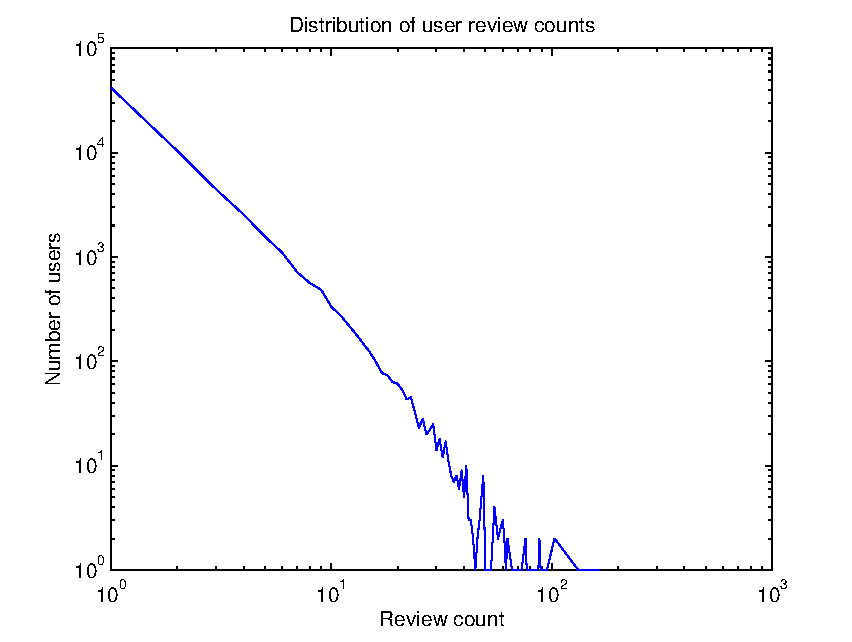
\includegraphics[width = 210pt]{images/u_hist.pdf}}
  \subfigure[small][Businesses]
            {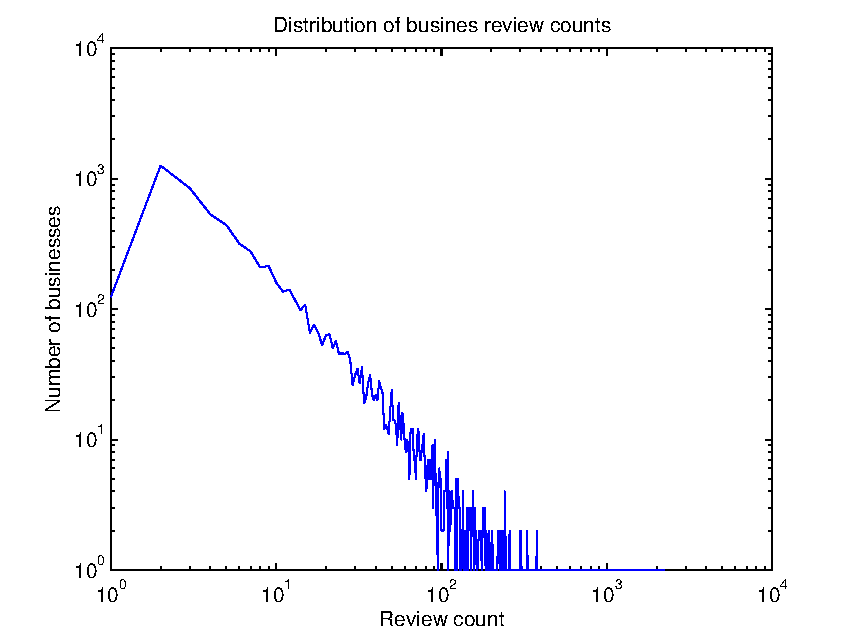
\includegraphics[width = 210pt]{images/b_hist.pdf}}

            \caption{Review count distributions}
            \label{review_count}

\end{figure}

\section{Neighborhood-based Collaborative Filtering}
In our first model, we use a neighborhood-based collaborative filtering method 
described as follows:
\begin{itemize}
\item For a given user $i$, calculate similarity between this users and all other
users. To compute similarity, we represent the dataset as a sparse matrix
of businesses and users, with values in the matrix being the ratings
assigned by the users to the businesses. We then take the cosine similarity
between the vectors of two users.
\item Select the k nearest neighbors of i based on this similarity measure
\item Compute a predicted rating for i based on a weighted combination of the
  nearest ratings neighbors
\end{itemize}

We used leave-1-out for our testing, training on all examples but the one
we tested on. With our first implementation of the model, we discovered a severe
limitation with our dataset - with the median number of ratings per user
being 1, more than half the users would not have another rating once we
removed the one for testing. 

To account for this, we predicted the rating for these users to be 4,
given that 4 was the median star rating in our dataset. We compare to a
baseline where 4 is predicted as the value for every star rating, and find
that our model significantly improves the root-mean-square error, as shown
in Table \ref{ncf}.

\begin{table}[htb]
\centering
\begin{tabular}{|c|c|}
\hline
{\bf Model} &{\bf RMSE} \tabularnewline \hline
Neighborhood-based CF &0.2032 \tabularnewline
Baseline (predict 4) &0.3454
\tabularnewline \hline

\end{tabular}
\caption{ Model Performance }
\label{ncf}
\end{table}

\section{Item-based Collaborative Filtering}
We attempted an implementation of item-based collaborative
filtering, based on the following steps:

\begin{itemize}
\item When considering the (user, business) pair, we calculate similarities
  between the target business and each of the businesses the user has
  rated previously
\item We use the cosine similarity metrics, and
  use all of the ratings for a particular business over the user space as
  a feature vector.
\item We find the k nearest neighbors to the target business from among
  the set of businesses the user has rated previously
\item Finally, we take a weighted average of the selected k businesses to
  compute a prediction of the rating for the target business 
\end{itemize}

However, this is not an ideal method for our dataset given its
sparsity. It is rendered useless when a user has a single review, and is
almost futile when a user has fewer than k reviews, as in that case, we
would simply be using as our prediction the average of the ratings
given by the user to all other businesses he has rated. In our results,
we found that the baseline of predicting the median 4 for all ratings
performed better than this model with any setting of k. 

For our final work, we may choose to either dismiss this model completely,
given its unsuitability for the limited dataset, test these algorithms on
an alternative dataset, or create a hybrid approach to account for the
sparsity of the data.

\section{Future Work}

For our final version, we intend to implement a version of Model-based
collaborative filtering, the final model of the three we had suggested
originally. In addition, we intend to rerun some of the models we have
already worked on with normalization and tweaks to account for data
sparsity.

For instance, in our version of neighborhood-based collaborative
filtering, we do not account for the number of common businesses reviewed
by two users when computing our metrics. As a result, two users who have a
single restaurant in common and rated it the same will be considered more
similar than two users who have 5 restaurants in common, rate 4 the same
and differ by a score of 1 point on the fifth. As the cosine similarity
metric uses a pure product of vector magnitudes in its denominator, we get
heavy biases against people who have a lot of reviews. We need to
find a way to account for this effect, while preventing the occurrence of
the opposite effect in which a pair of users with only a single
intersecting business are viewed as more similar than those with many
intersecting businesses.

Finally, if time permits, we intend to move our methods onto a different
data set. With the two methods we have implemented so far, we have seen
that the sparsity of our current dataset puts us at a large disadvantage
and produces poor results. Thus, it would be interesting to compare the
performances of these techniques on a dataset which contains more edges
between the various nodes.


\end{document}
